\documentclass[conference]{IEEEtran}
\usepackage{iftex}
\ifXeTeX
  \usepackage{fontspec}
  \setmainfont{texgyretermes}[Extension=.otf,UprightFont=*-regular,BoldFont=*-bold,ItalicFont=*-italic,BoldItalicFont=*-bolditalic]
  \setmonofont{texgyrecursor}[Extension=.otf,UprightFont=*-regular,BoldFont=*-bold,ItalicFont=*-italic,BoldItalicFont=*-bolditalic]
\else
  \usepackage[utf8]{inputenc}
  \usepackage[T1]{fontenc}
  \usepackage{newtxtext,newtxmath}
\fi
\usepackage{amsmath,amssymb}
\usepackage{graphicx}
\usepackage{booktabs}
\usepackage{array}
\usepackage{url}
\usepackage[hidelinks]{hyperref}
\usepackage{xcolor}
\graphicspath{{figures/}}
% Generated by analysis/make_numbers.py. Do not edit by hand.
\newcommand{\AblDropcontention}{0.20}
\newcommand{\AblDropneedpressure}{0.25}
\newcommand{\AblDroprequestrate}{0.22}
\newcommand{\AblDropscarcity}{0.26}
\newcommand{\AblDropwaitingratio}{0.27}
\newcommand{\AblEqual}{0.24}
\newcommand{\AvailF}{0.16}
\newcommand{\AvailFA}{0.71}
\newcommand{\AvailFAsub}{0.35}
\newcommand{\AvailFDlp}{0.05}
\newcommand{\AvailFHFifty}{0.25}
\newcommand{\AvailFHFive}{0.06}
\newcommand{\AvailFHTen}{0.10}
\newcommand{\AvailFHTwenty}{0.16}
\newcommand{\AvailFNormal}{0.10}
\newcommand{\AvailFSpike}{0.34}
\newcommand{\AvailFdl}{0.16}
\newcommand{\AvailFdlL}{0.29}
\newcommand{\AvailFhi}{0.16}
\newcommand{\AvailFhisub}{0.30}
\newcommand{\AvailFlo}{0.16}
\newcommand{\AvailFlosub}{0.29}
\newcommand{\AvailFsub}{0.30}
\newcommand{\AvailK}{1}
\newcommand{\AvailLead}{8}
\newcommand{\AvailLeadDlp}{8}
\newcommand{\AvailLeadFive}{0.72}
\newcommand{\AvailLeadFivesub}{0.49}
\newcommand{\AvailLeadNormal}{10}
\newcommand{\AvailLeadSpike}{7}
\newcommand{\AvailLeadsub}{4}
\newcommand{\AvailP}{0.11}
\newcommand{\AvailPsub}{0.48}
\newcommand{\AvailR}{0.34}
\newcommand{\AvailRdl}{0.52}
\newcommand{\AvailRdlL}{0.55}
\newcommand{\AvailRf}{20}
\newcommand{\AvailRsub}{0.22}
\newcommand{\AvailTh}{95}
\newcommand{\AwsCost}{4.11}
\newcommand{\AwsHours}{2.9}
\newcommand{\AwsWall}{2 h 43 min}
\newcommand{\CPUs}{32}
\newcommand{\CombF}{0.28}
\newcommand{\CombFA}{0.33}
\newcommand{\CombFAsub}{0.48}
\newcommand{\CombFDlp}{0.23}
\newcommand{\CombFHFifty}{0.40}
\newcommand{\CombFHFive}{0.11}
\newcommand{\CombFHTen}{0.19}
\newcommand{\CombFHTwenty}{0.28}
\newcommand{\CombFNormal}{0.22}
\newcommand{\CombFSpike}{0.42}
\newcommand{\CombFdl}{0.33}
\newcommand{\CombFdlL}{0.53}
\newcommand{\CombFhi}{0.28}
\newcommand{\CombFhisub}{0.45}
\newcommand{\CombFlo}{0.28}
\newcommand{\CombFlosub}{0.44}
\newcommand{\CombFsub}{0.44}
\newcommand{\CombK}{1}
\newcommand{\CombLead}{10}
\newcommand{\CombLeadDlp}{11}
\newcommand{\CombLeadFive}{0.75}
\newcommand{\CombLeadFivesub}{0.56}
\newcommand{\CombLeadNormal}{12}
\newcommand{\CombLeadSpike}{7}
\newcommand{\CombLeadsub}{5}
\newcommand{\CombP}{0.24}
\newcommand{\CombPsub}{0.56}
\newcommand{\CombR}{0.34}
\newcommand{\CombRdl}{0.71}
\newcommand{\CombRdlL}{0.76}
\newcommand{\CombRf}{10}
\newcommand{\CombRsub}{0.37}
\newcommand{\CombTh}{65}
\newcommand{\CombW}{double\_contention}
\newcommand{\ContF}{0.34}
\newcommand{\ContFA}{0.22}
\newcommand{\ContFAsub}{1.04}
\newcommand{\ContFDlp}{0.22}
\newcommand{\ContFHFifty}{0.43}
\newcommand{\ContFHFive}{0.13}
\newcommand{\ContFHTen}{0.22}
\newcommand{\ContFHTwenty}{0.34}
\newcommand{\ContFNormal}{0.21}
\newcommand{\ContFSpike}{0.49}
\newcommand{\ContFdl}{0.26}
\newcommand{\ContFdlL}{0.44}
\newcommand{\ContFhi}{0.34}
\newcommand{\ContFhisub}{0.52}
\newcommand{\ContFlo}{0.34}
\newcommand{\ContFlosub}{0.51}
\newcommand{\ContFsub}{0.51}
\newcommand{\ContK}{1}
\newcommand{\ContLead}{7}
\newcommand{\ContLeadDlp}{9}
\newcommand{\ContLeadFive}{0.69}
\newcommand{\ContLeadFivesub}{0.61}
\newcommand{\ContLeadNormal}{9}
\newcommand{\ContLeadSpike}{7}
\newcommand{\ContLeadsub}{6}
\newcommand{\ContP}{0.30}
\newcommand{\ContPsub}{0.46}
\newcommand{\ContR}{0.39}
\newcommand{\ContRdl}{0.54}
\newcommand{\ContRdlL}{0.58}
\newcommand{\ContRf}{20}
\newcommand{\ContRsub}{0.59}
\newcommand{\ContTh}{60}
\newcommand{\EpDeadDlp}{100}
\newcommand{\EpDeadNormal}{77}
\newcommand{\EpDeadSpike}{100}
\newcommand{\EpNDlp}{31{,}219}
\newcommand{\EpNNormal}{21{,}525}
\newcommand{\EpNSpike}{29{,}868}
\newcommand{\EpRecDlp}{0}
\newcommand{\EpRecNormal}{23}
\newcommand{\EpRecSpike}{0}
\newcommand{\GitCommit}{d3de8e5}
\newcommand{\LookCost}{39}
\newcommand{\LookCostN}{200}
\newcommand{\LookF}{0.74}
\newcommand{\LookFA}{0.62}
\newcommand{\LookFAsub}{0.62}
\newcommand{\LookFDlp}{0.69}
\newcommand{\LookFHFifty}{0.80}
\newcommand{\LookFHFive}{0.48}
\newcommand{\LookFHTen}{0.65}
\newcommand{\LookFHTwenty}{0.74}
\newcommand{\LookFNormal}{0.66}
\newcommand{\LookFSpike}{0.83}
\newcommand{\LookFdl}{0.37}
\newcommand{\LookFdlL}{0.76}
\newcommand{\LookFhi}{0.75}
\newcommand{\LookFhisub}{0.75}
\newcommand{\LookFlo}{0.74}
\newcommand{\LookFlosub}{0.74}
\newcommand{\LookFsub}{0.74}
\newcommand{\LookK}{1}
\newcommand{\LookLead}{4}
\newcommand{\LookLeadDlp}{8}
\newcommand{\LookLeadFive}{0.48}
\newcommand{\LookLeadFivesub}{0.48}
\newcommand{\LookLeadNormal}{6}
\newcommand{\LookLeadSpike}{3}
\newcommand{\LookLeadsub}{4}
\newcommand{\LookP}{0.69}
\newcommand{\LookPsub}{0.69}
\newcommand{\LookR}{0.81}
\newcommand{\LookRdl}{0.43}
\newcommand{\LookRdlL}{0.81}
\newcommand{\LookRf}{10}
\newcommand{\LookRsub}{0.81}
\newcommand{\LookTh}{30}
\newcommand{\Machine}{c7i.8xlarge}
\newcommand{\MaxN}{200}
\newcommand{\NEventsTest}{82{,}612}
\newcommand{\NSeedsPerCell}{10{,}000}
\newcommand{\NSeqAll}{300{,}000}
\newcommand{\NSeqTest}{150{,}000}
\newcommand{\NSeqTune}{150{,}000}
\newcommand{\NSizes}{5}
\newcommand{\NStepsAllM}{676.2}
\newcommand{\NStepsTest}{338{,}262{,}425}
\newcommand{\NStepsTune}{337{,}917{,}758}
\newcommand{\NeedF}{0.19}
\newcommand{\NeedFA}{0.07}
\newcommand{\NeedFAsub}{0.08}
\newcommand{\NeedFDlp}{0.01}
\newcommand{\NeedFHFifty}{0.22}
\newcommand{\NeedFHFive}{0.08}
\newcommand{\NeedFHTen}{0.13}
\newcommand{\NeedFHTwenty}{0.19}
\newcommand{\NeedFNormal}{0.06}
\newcommand{\NeedFSpike}{0.34}
\newcommand{\NeedFdl}{0.23}
\newcommand{\NeedFdlL}{0.36}
\newcommand{\NeedFhi}{0.19}
\newcommand{\NeedFhisub}{0.19}
\newcommand{\NeedFlo}{0.19}
\newcommand{\NeedFlosub}{0.18}
\newcommand{\NeedFsub}{0.18}
\newcommand{\NeedK}{1}
\newcommand{\NeedLead}{7}
\newcommand{\NeedLeadDlp}{6}
\newcommand{\NeedLeadFive}{0.66}
\newcommand{\NeedLeadFivesub}{0.43}
\newcommand{\NeedLeadNormal}{8}
\newcommand{\NeedLeadSpike}{7}
\newcommand{\NeedLeadsub}{4}
\newcommand{\NeedP}{0.31}
\newcommand{\NeedPsub}{0.65}
\newcommand{\NeedR}{0.14}
\newcommand{\NeedRdl}{0.34}
\newcommand{\NeedRdlL}{0.36}
\newcommand{\NeedRf}{20}
\newcommand{\NeedRsub}{0.11}
\newcommand{\NeedTh}{95}
\newcommand{\PairAvailComb}{11}
\newcommand{\PairAvailEarlier}{60}
\newcommand{\PairAvailN}{16{,}754}
\newcommand{\PairAvailOther}{8}
\newcommand{\PairContComb}{9}
\newcommand{\PairContEarlier}{34}
\newcommand{\PairContN}{18{,}610}
\newcommand{\PairContOther}{8}
\newcommand{\PairLookComb}{5}
\newcommand{\PairLookEarlier}{48}
\newcommand{\PairLookN}{8{,}012}
\newcommand{\PairLookOther}{4}
\newcommand{\PairNeedComb}{10}
\newcommand{\PairNeedEarlier}{65}
\newcommand{\PairNeedN}{7{,}163}
\newcommand{\PairNeedOther}{7}
\newcommand{\PairRandComb}{10}
\newcommand{\PairRandEarlier}{42}
\newcommand{\PairRandN}{254}
\newcommand{\PairRandOther}{11}
\newcommand{\PairRateComb}{6}
\newcommand{\PairRateEarlier}{33}
\newcommand{\PairRateN}{6{,}113}
\newcommand{\PairRateOther}{8}
\newcommand{\PairWaitComb}{12}
\newcommand{\PairWaitEarlier}{49}
\newcommand{\PairWaitN}{8{,}926}
\newcommand{\PairWaitOther}{12}
\newcommand{\Platform}{Linux-7.0.0-1014-aws-x86\_64-with-glibc2.39}
\newcommand{\RamGB}{62}
\newcommand{\RandF}{0.01}
\newcommand{\RandFA}{0.43}
\newcommand{\RandFAsub}{0.42}
\newcommand{\RandFDlp}{0.01}
\newcommand{\RandFHFifty}{0.02}
\newcommand{\RandFHFive}{0.00}
\newcommand{\RandFHTen}{0.00}
\newcommand{\RandFHTwenty}{0.01}
\newcommand{\RandFNormal}{0.00}
\newcommand{\RandFSpike}{0.01}
\newcommand{\RandFdl}{0.01}
\newcommand{\RandFdlL}{0.02}
\newcommand{\RandFhi}{0.01}
\newcommand{\RandFhisub}{0.01}
\newcommand{\RandFlo}{0.01}
\newcommand{\RandFlosub}{0.01}
\newcommand{\RandFsub}{0.01}
\newcommand{\RandLead}{11}
\newcommand{\RandLeadDlp}{11}
\newcommand{\RandLeadFive}{0.82}
\newcommand{\RandLeadFivesub}{0.79}
\newcommand{\RandLeadNormal}{11}
\newcommand{\RandLeadSpike}{11}
\newcommand{\RandLeadsub}{9}
\newcommand{\RandP}{0.45}
\newcommand{\RandPsub}{0.03}
\newcommand{\RandR}{0.01}
\newcommand{\RandRdl}{0.01}
\newcommand{\RandRdlL}{0.02}
\newcommand{\RandRsub}{0.01}
\newcommand{\RateF}{0.14}
\newcommand{\RateFA}{0.15}
\newcommand{\RateFAsub}{0.52}
\newcommand{\RateFDlp}{0.00}
\newcommand{\RateFHFifty}{0.23}
\newcommand{\RateFHFive}{0.04}
\newcommand{\RateFHTen}{0.08}
\newcommand{\RateFHTwenty}{0.14}
\newcommand{\RateFNormal}{0.00}
\newcommand{\RateFSpike}{0.23}
\newcommand{\RateFdl}{0.06}
\newcommand{\RateFdlL}{0.13}
\newcommand{\RateFhi}{0.14}
\newcommand{\RateFhisub}{0.34}
\newcommand{\RateFlo}{0.13}
\newcommand{\RateFlosub}{0.33}
\newcommand{\RateFsub}{0.33}
\newcommand{\RateK}{3}
\newcommand{\RateLead}{9}
\newcommand{\RateLeadDlp}{11}
\newcommand{\RateLeadFive}{0.75}
\newcommand{\RateLeadFivesub}{0.71}
\newcommand{\RateLeadNormal}{10}
\newcommand{\RateLeadSpike}{9}
\newcommand{\RateLeadsub}{8}
\newcommand{\RateP}{0.16}
\newcommand{\RatePsub}{0.44}
\newcommand{\RateR}{0.12}
\newcommand{\RateRdl}{0.06}
\newcommand{\RateRdlL}{0.12}
\newcommand{\RateRf}{20}
\newcommand{\RateRsub}{0.27}
\newcommand{\RateTh}{95}
\newcommand{\SafetyUsMax}{34.9}
\newcommand{\ScaleMaxN}{200}
\newcommand{\SlopeRef}{0.77}
\newcommand{\SlopeVec}{0.29}
\newcommand{\SpeedupMax}{7.7}
\newcommand{\SpeedupMin}{1.3}
\newcommand{\SpikeBefore}{3.0}
\newcommand{\SpikeMedSteps}{26}
\newcommand{\WaitF}{0.25}
\newcommand{\WaitFA}{0.31}
\newcommand{\WaitFAsub}{0.32}
\newcommand{\WaitFDlp}{0.31}
\newcommand{\WaitFHFifty}{0.34}
\newcommand{\WaitFHFive}{0.09}
\newcommand{\WaitFHTen}{0.17}
\newcommand{\WaitFHTwenty}{0.25}
\newcommand{\WaitFNormal}{0.29}
\newcommand{\WaitFSpike}{0.03}
\newcommand{\WaitFdl}{0.48}
\newcommand{\WaitFdlL}{0.65}
\newcommand{\WaitFhi}{0.25}
\newcommand{\WaitFhisub}{0.15}
\newcommand{\WaitFlo}{0.25}
\newcommand{\WaitFlosub}{0.14}
\newcommand{\WaitFsub}{0.14}
\newcommand{\WaitK}{1}
\newcommand{\WaitLead}{13}
\newcommand{\WaitLeadDlp}{13}
\newcommand{\WaitLeadFive}{0.86}
\newcommand{\WaitLeadFivesub}{0.48}
\newcommand{\WaitLeadNormal}{13}
\newcommand{\WaitLeadSpike}{5}
\newcommand{\WaitLeadsub}{4}
\newcommand{\WaitP}{0.24}
\newcommand{\WaitPsub}{0.32}
\newcommand{\WaitR}{0.26}
\newcommand{\WaitRdl}{0.83}
\newcommand{\WaitRdlL}{0.83}
\newcommand{\WaitRf}{10}
\newcommand{\WaitRsub}{0.09}
\newcommand{\WaitTh}{90}
\newcommand{\WithEventDlp}{62}
\newcommand{\WithEventNormal}{35}
\newcommand{\WithEventSpike}{60}


\begin{document}

\title{Predictive Deadlock Warning: Early Detection of Unsafe States from Resource-Request Patterns}

\author{\IEEEauthorblockN{Revanth Reddy Lingala and Padigela Srujan}
\IEEEauthorblockA{Department of Information Technology\\
Chaitanya Bharathi Institute of Technology (CBIT), Hyderabad, India}}

\maketitle

\begin{abstract}
Banker's algorithm tells an operating system whether the current resource-allocation state is \emph{safe}; it gives no signal that the system is drifting towards an unsafe state. We ask how early, and how reliably, an unsafe state can be anticipated before the safety check reports it, and at what computational cost. We propose an explainable, rule-based early-warning score that combines five resource-pressure indicators with a persistence and refractory rule, and we compare it with a free-resource threshold, each indicator alone, a weighted-maximum variant, logistic regression and gradient-boosted trees trained on the same signals, a scalar safety margin in the spirit of Finkel and Madduri, a cheap top-3 lookahead, and an exact one-step lookahead that tests every running process. An observer-mode simulator grants every valid request so that unsafe states actually occur, and records Banker's safety and deadlock-detection outcomes after every step. Evaluation follows event-based early-warning practice: alarm precision, event recall, lead time, refractory periods, censoring, an NAB-style early-detection score and stratified bootstrap confidence intervals, with tuning and test on disjoint seeds. Over \NSeqAll{} simulated sequences (\NStepsAllM{} million requests) on AWS EC2, the rule-based score reached F1 = \CombF{} [\CombFlo, \CombFhi] with a median warning of \CombLead{} steps, against \AvailF{} for the free-resource threshold and \RandF{} for random alarms at a matched rate; gradient-boosted trees trained on the \emph{same} cheap signals reached \GbtF{} with a median warning of \GbtLead{} steps, while logistic regression gained little (\LrF), so non-linear interactions between the signals carry much of the missing information. State-based checks were more accurate still: on the sequences where all methods were computed, a scalar safety margin reached \MargFsub{} against \LookFsub{} for exact lookahead, at \MargCostMaxN{} versus \LookCostMaxN{} times the compute of a simulation step for 200 processes, but warned later. Results were insensitive to maximum claims misdeclared by $\pm$20\%, and unsafe episodes overwhelmingly ended in deadlock. Together the methods map a cost--accuracy--lead-time frontier for anticipating Banker's verdict.
\end{abstract}

\begin{IEEEkeywords}
deadlock avoidance, Banker's algorithm, early warning, resource allocation, operating systems, event-based evaluation
\end{IEEEkeywords}

% ===================================================================
\section{Introduction}
Deadlock---processes holding resources while waiting for resources held by each other---remains a practical hazard wherever resources are allocated incrementally. Cluster schedulers that place the tasks of a gang-structured job one at a time can leave several jobs each holding part of what they need, a ``temporary deadlock'' reported in deep-learning platforms~\cite{Jayaram2019FfDL,Lin2019DRAGON} and the motivation for all-or-nothing placement in recent Kubernetes releases~\cite{K8sBlog2025}. Resource exhaustion more broadly is a recurring cause of cloud outages~\cite{Gunawi2016}.

The classical avoidance method, Banker's algorithm~\cite{Dijkstra-EWD123,Dijkstra-EWD623,Habermann1969}, checks whether a state is \emph{safe}: whether some order exists in which every process can obtain its remaining maximum claim and finish. The check is binary and present-tense. It says \emph{safe now} or \emph{unsafe now}, but nothing about whether the system is drifting towards the boundary, and it is seldom used in practice because of its cost~\cite{Belik1987}. Operations teams, meanwhile, rely on early alerts that page before a resource saturates~\cite{Ewaschuk2016SRE}.

Prior work has made this check faster~\cite{Belik1987,Finkel1987,Zohora2024}, characterised its computational complexity~\cite{Gold1978,Minoura1982}, detected deadlocks after they form~\cite{Agrawal1983,Chandy1983}, or predicted different kinds of deadlock, such as lock-order bugs in programs~\cite{Tunc2023} or virtual-machine overload~\cite{LeNgoc2023}. In all of it, the safety question remains present-tense. This paper asks a complementary, forward-looking question---analogous to a smoke detector that sounds before the fire alarm: \emph{how early, how reliably and at what cost can an unsafe state be anticipated before Banker's algorithm reports it?} We study eight research questions:
\begin{itemize}
\item RQ1: Do indicators computed from the allocation state and request stream anticipate unsafe states?
\item RQ2: How much lead time do alarms provide?
\item RQ3: What alarm precision and event recall do they achieve?
\item RQ4: Which indicators matter, how should they be combined, and do learned models on the same signals do better?
\item RQ5: How does warning quality vary across workloads?
\item RQ6: How often do unsafe states become deadlocks, and can alarms anticipate deadlocks?
\item RQ7: What does each method cost, and how does the safety check scale?
\item RQ8: How robust are the indicators when maximum claims are misdeclared?
\end{itemize}

\textbf{Contributions.} (i) An explainable, rule-based early-warning score for Banker's unsafe states, with no trained model. (ii) An observer-mode simulator with three controlled workloads, verified by 133 unit and property tests. (iii) An event-based evaluation protocol adapted from clinical, seismic and anomaly-detection early warning~\cite{Hyland2020,Munchmeyer2021,Tatbul2018,Lavin2015}. (iv) A broad baseline set---matched-rate random alarms, a free-resource threshold, single indicators, learned models, a scalar safety margin, a cheap top-$k$ lookahead and exact lookahead---that maps the \emph{cost--accuracy frontier} for anticipating Banker's verdict. (v) A separate measurement of unsafe and deadlocked outcomes, a robustness study with misdeclared claims, and a scaling study, all run at scale on AWS EC2.

% ===================================================================
\section{Background}
\subsection{Deadlock and Banker's algorithm}
A system has $m$ resource types with $\mathit{total}_j$ units each and $n$ processes. Process $i$ declares a maximum claim $\mathit{Max}_{ij}$, holds $\mathit{Alloc}_{ij}$ and may still request $\mathit{Need}_{ij}=\mathit{Max}_{ij}-\mathit{Alloc}_{ij}$; free units are $\mathit{Avail}_j=\mathit{total}_j-\sum_i\mathit{Alloc}_{ij}$. Deadlock requires mutual exclusion, hold-and-wait, no preemption and circular wait~\cite{Coffman1971}; graph models and reduction-based detection are due to Holt~\cite{Holt1972}. In Banker's algorithm~\cite{Dijkstra-EWD623,Habermann1969}, a state is safe if a sequence exists in which each process's need fits the free units plus everything released by the processes before it. The banker grants a request only if the resulting state is safe. The textbook safety check~\cite{Silberschatz2018,Tanenbaum2022} costs $\Theta(mn^2)$~\cite{Belik1987}.

\subsection{Unsafe is not deadlock}
The safety check is pessimistic: it assumes every process may request its full remaining claim. Deadlock detection is optimistic: it assumes running processes finish and release everything, so only blocked processes' pending requests matter~\cite{Holt1972,Silberschatz2018}. A state can be safe and not deadlocked, unsafe and not deadlocked, or unsafe and deadlocked, but never safe and deadlocked; safety is also not sufficient for liveness, since processes can still be postponed indefinitely~\cite{Holt1971,ParnasHabermann1972}. We therefore record both outcomes at every step and treat the unsafe onset as the primary prediction target and the deadlock onset as a secondary one.

% ===================================================================
\section{Literature Survey and Positioning}
We organise prior work into seven themes, then state precisely where our work sits (Table~\ref{tab:positioning}).

\subsection{Foundations: Banker's algorithm and the notion of safety}
Deadlock handling is classically split into prevention, avoidance and detection~\cite{Coffman1971,Holt1972}. Prevention removes one of the four necessary conditions, for example by imposing a global order on resource acquisition~\cite{Havender1968}. Avoidance, our setting, originates with Dijkstra's Banker's algorithm~\cite{Dijkstra-EWD123,Dijkstra-EWD623}, generalised to multiple resource types by Habermann~\cite{Habermann1969}. Holt, and Parnas and Habermann, showed that safety guarantees deadlock freedom but not freedom from indefinite postponement~\cite{Holt1971,ParnasHabermann1972}. \emph{Relevance:} Dijkstra's definition of a safe state---a completion order exists in which every process obtains its remaining claim---is the exact ground truth our warnings try to anticipate. Every alarm, metric and baseline in this paper is defined relative to the moment this test first fails, so the original formulation is the reference point of the whole evaluation, not historical background.

\subsection{Theory of deadlock prediction and avoidance}
In the classical theory, ``deadlock prediction'' means deciding, from the current status of a resource allocation system, whether deadlock is still avoidable---the question Banker's algorithm answers. Gold showed that this decision is polynomial for reusable resources without partial requests (Banker's case) and NP-complete when either restriction is lifted~\cite{Gold1978}. Minoura developed avoidance algorithms that admit more concurrency than Havender's and Habermann's schemes and showed that avoidance for processes with branches is PSPACE-complete~\cite{Minoura1982}. Kameda tested whether free-running processes can ever become deadlocked using network flow~\cite{Kameda1980}. \emph{Difference:} all of these works decide a \emph{static, present-tense} property of a state---is it, or can it become, deadlocked or unsafe? We instead forecast \emph{when} a running system will cross from safe to unsafe, from the trajectory of the allocation state, and measure how early and how reliably that crossing can be signalled.

\subsection{Faster and dynamic safety tests}
Because the safety check costs $\Theta(mn^2)$, most follow-up work makes it cheaper. Belik obtained an amortised $O(mn)$ variant under likely conditions and noted that avoidance is ``seldom used on account of its high cost''~\cite{Belik1987}. Finkel and Madduri maintain safe sequences between allocator calls for an $O(\log n)$ test and compute the minimum resources a state needs to remain safe~\cite{Finkel1987}. Li and Cook give near-linear detection algorithms when resource types are few~\cite{LiCook2007}, Lang extends the algorithm's applicability~\cite{Lang1999}, and DBDAA admits processes dynamically and speeds up safe-state determination~\cite{Zohora2024}. Andrews and Levin evaluate the safety of prospective requests between requests~\cite{AndrewsLevin1982}. \emph{Difference:} these works answer the same binary question faster; none anticipates the verdict. Two of them directly inspire our strongest baselines: our safety margin is a scalar, proportional form of Finkel and Madduri's minimum resources to remain safe, and our lookahead baselines follow Andrews and Levin's idea of testing prospective requests. We go beyond them by measuring what such checks buy as \emph{early-warning signals} and what they cost.

\subsection{Deadlock detection in databases and distributed systems}
Practical systems often detect and recover instead of avoiding. In databases a deadlock is a cycle in the waits-for graph and can be detected cheaply~\cite{Agrawal1983,Knapp1987}; distributed detection uses probe messages along wait-for edges~\cite{Chandy1983,Singhal1989}. \emph{Difference:} detection reports a deadlock after it has formed; we warn before the system even becomes unsafe, and we report how often unsafe states actually turn into detected deadlocks.

\subsection{Deadlock control beyond operating systems}
Deadlock avoidance and prevention are mature in automated manufacturing, where Petri-net models of shared machines and buffers yield avoidance and prevention policies~\cite{Banaszak1990,Ezpeleta1995,Fanti2004,Li2008}. Cluster managers allocate multi-dimensional resources to many concurrent jobs at datacentre scale~\cite{Verma2015}, and the hold-and-wait pattern reappears there: deep-learning platforms report ``temporary deadlocks'' when gang jobs are placed task by task~\cite{Jayaram2019FfDL,Lin2019DRAGON}, motivating all-or-nothing placement in Kubernetes~\cite{K8sBlog2025}, and load problems are a recurring cause of cloud outages~\cite{Gunawi2016}. \emph{Relevance:} these works show the problem is not confined to textbooks and motivate our spike workload. \emph{Difference:} they design control policies; we study prediction of the unsafe boundary and its cost.

\subsection{Deadlock prediction in programs and learning-based prediction}
In programming languages, ``deadlock prediction'' means finding lock-order deadlocks that some reordering of an observed execution could exhibit: lock-graph analysis~\cite{Bensalem2006}, randomised active testing~\cite{Joshi2009}, sound prediction~\cite{Kalhauge2018} and sound online prediction in linear time~\cite{Tunc2023}. \emph{Difference:} these tools find bugs in program code, involve single-unit locks with no declared claims, and answer whether a deadlock is \emph{possible} in some interleaving; we monitor a running multi-unit resource allocator and forecast an imminent unsafe state. On the resource side, Le~Ngoc and Tran~Cong use linear regression in CloudSim to forecast virtual-machine ``deadlock'' for load balancing~\cite{LeNgoc2023}; deadlock there means overload rather than Banker's unsafety, and neither lead time nor event-level precision is reported. AI-based thread-deadlock prediction has been proposed in preprints without empirical evaluation~\cite{Oluwaseyi2024}. More broadly, failure prediction~\cite{Salfner2010} and anomaly detection~\cite{Chandola2009} learn to flag abnormal system states; our learned baselines use gradient boosting~\cite{Friedman2001} on the same signals as our rule.

\subsection{How early warnings are evaluated}
A warning system must be judged on whether alarms come \emph{before} events and how many are false---not on per-step accuracy, which a silent detector maximises when events are rare. Online failure prediction frames this through lead time and prediction windows~\cite{Salfner2010}. \emph{Relevance of clinical early warning:} Hyland et al.\ predict circulatory failure in intensive care with exactly our problem structure---a rare, harmful state change, a continuously monitored state, and value only if the alarm comes early~\cite{Hyland2020}. They define event-level recall (events preceded by an alarm within a window), alarm-level precision (alarms followed by an event) and a silencing period after each alarm; we adopt these three definitions directly, and their reported operating point (about 30\% precision) calibrates what ``moderate'' precision means for rare-event warning. \emph{Relevance of seismic early warning:} Münchmeyer et al.\ evaluate earthquake alerts by alert quality \emph{together with} warning time and show that lowering the alert threshold buys warning time at the cost of precision~\cite{Munchmeyer2021}; this is why we report precision against lead time along every threshold sweep (Fig.~\ref{fig:leadprec}) and treat an alarm at the onset as a miss. Range-based precision and recall~\cite{Tatbul2018} and the Numenta Anomaly Benchmark score~\cite{Lavin2015} motivate treating unsafe episodes as ranges and rewarding earlier detection. Because onsets are rare we use precision--recall rather than ROC analysis~\cite{Saito2015,Davis2006}, and bootstrap confidence intervals over whole sequences~\cite{Efron1993}. No deadlock study we found evaluates warnings this way, which is why these references come from medicine and seismology.

\subsection{Positioning and novelty}
Table~\ref{tab:positioning} compares the closest prior work with ours. Prior work either decides safety or deadlock-freedom for the current state~\cite{Gold1978,Minoura1982,Kameda1980}, decides it faster~\cite{Belik1987,Finkel1987,Zohora2024}, detects deadlocks after they form~\cite{Agrawal1983,Chandy1983}, predicts a different kind of deadlock (lock-order bugs in programs~\cite{Kalhauge2018,Tunc2023} or VM overload~\cite{LeNgoc2023}), or controls deadlock in other domains~\cite{Ezpeleta1995,Li2008}. To our knowledge, this is the first work to (i) forecast the safe-to-unsafe transition of a Banker-style resource allocator before the safety check fires, (ii) evaluate that forecast with event-based precision, recall and lead time against matched-rate random, threshold, learned and exact-lookahead baselines, and (iii) quantify the trade-off between accuracy, lead time and compute cost, including a cheap safety margin that nearly matches exact lookahead.

\begin{table*}[t]
\centering
\footnotesize
\caption{Positioning against the closest prior work. ``Forecast'' = predicts a \emph{future} transition rather than deciding a property of the current state.}
\label{tab:positioning}
\begin{tabular}{>{\raggedright\arraybackslash}p{3.3cm}>{\raggedright\arraybackslash}p{3.7cm}>{\raggedright\arraybackslash}p{2.5cm}cccc}
\toprule
Work & Problem & Target & Forecast & Lead time & Event-based eval. & Cost analysis \\
\midrule
Dijkstra; Habermann~\cite{Dijkstra-EWD623,Habermann1969} & Avoidance: is the state safe? & Banker's safety & -- & -- & -- & -- \\
Gold; Minoura~\cite{Gold1978,Minoura1982} & Complexity of deadlock prediction & avoidability & -- & -- & -- & complexity \\
Belik; Finkel \& Madduri; DBDAA~\cite{Belik1987,Finkel1987,Zohora2024} & Faster safety tests & Banker's safety & -- & -- & -- & \checkmark \\
Agrawal et al.; Chandy et al.~\cite{Agrawal1983,Chandy1983} & Deadlock detection & formed deadlock & -- & -- & -- & \checkmark \\
Kalhauge \& Palsberg; Tun\c{c} et al.~\cite{Kalhauge2018,Tunc2023} & Lock deadlocks in program traces & possible bug & -- & -- & -- & \checkmark \\
Le Ngoc \& Tran Cong~\cite{LeNgoc2023} & ML load balancing in CloudSim & VM overload & \checkmark & -- & -- & -- \\
Ezpeleta et al.; Li et al.~\cite{Ezpeleta1995,Li2008} & Petri-net deadlock control (manufacturing) & deadlock-free policy & -- & -- & -- & -- \\
Hyland et al.; Münchmeyer et al.~\cite{Hyland2020,Munchmeyer2021} & Clinical / seismic early warning & patient / earthquake event & \checkmark & \checkmark & \checkmark & -- \\
\textbf{This work} & \textbf{Early warning of Banker-unsafe states} & \textbf{unsafe (and deadlock) onset} & \checkmark & \checkmark & \checkmark & \checkmark \\
\bottomrule
\end{tabular}
\end{table*}

% ===================================================================
\section{Simulator}
\subsection{Observer mode}
If Banker's algorithm refused unsafe requests, the system would never become unsafe and nothing could be predicted. Our simulator therefore grants every valid request and uses Banker's algorithm only to \emph{observe}. Each step: (1) waiting processes are retried first-come first-served, and any process whose claim is now met finishes and releases everything, repeating until nothing changes; (2) one active, non-waiting process issues a non-zero request no larger than its need, which is granted if it fits the free units and otherwise blocks the process with the request pending; (3) completed processes release their resources; (4) in the \textit{normal} workload a process may release part of its allocation early; (5) the simulator records whether the state is unsafe, whether it is deadlocked, the five indicators and the state-based baselines. A sequence ends at the first deadlock, when all processes finish, or at a step cap. Because no request is refused, observer mode also avoids a confound of clinical early warning, where interventions prevent events and turn correct alarms into apparent false positives~\cite{Hyland2020}.

\subsection{Correctness}
Initial states are regenerated until safe. Invariants---conservation of units, allocation $\le$ claim, pending $\le$ need, finished processes hold nothing---are asserted in a debug mode used by the tests. A vectorised NumPy safety check, which finishes every process that fits in each pass, agrees with the textbook loop on 2,000 random states, as does deadlock detection; both reproduce the textbook examples of~\cite{Silberschatz2018}. The property \emph{deadlocked $\Rightarrow$ unsafe} holds on every random state tested. Since detection assumes non-waiting processes release everything, grants to, releases by and completions of such processes cannot change its result; detection therefore reruns only when the waiting set or a pending request changes, which we verified against every-step detection. Recording the extra baselines draws on a separate random stream, so the simulated workload is identical with or without them. In total 133 tests cover every row of our edge-case matrix.

\subsection{Workloads}
Requests are fractions of remaining need, so behaviour is comparable across sizes. The main calibration parameter is claim tightness, $\sum_i\mathit{Max}_{ij}/\mathit{total}_j$. \textit{Normal}: small single-resource requests and occasional partial releases. \textit{Spike}: normal traffic, then---once a random 20--60\% of the initial total need has been requested---80\% of processes make broad grabs of 30--60\% of their remaining need, capped by free units and holding back the last unit, a pattern akin to piecewise gang placement~\cite{Jayaram2019FfDL}. \textit{Deadlock-prone}: process $i$ prefers resource $(i{+}1)\bmod m$, inducing circular wait~\cite{Coffman1971}, and rarely takes its final unit. Parameters were calibrated on tuning seeds only so that each workload yields a mix of sequences with and without unsafe events (\WithEventNormal\%, \WithEventSpike\% and \WithEventDlp\% of test sequences contain at least one, averaged over sizes).

% ===================================================================
\section{Warning Methods}
\subsection{Rule-based score}
After every step five indicators in $[0,1]$ are computed: \emph{scarcity} $=1-\sum_j\mathit{Avail}_j/\sum_j\mathit{total}_j$; \emph{need pressure} $=\frac{1}{m}\sum_j S_j/(S_j+\mathit{Avail}_j)$, with $S_j$ the outstanding need of active processes; \emph{contention}, the fraction of resource types for which at least two active processes need more than is free; \emph{waiting ratio}, the fraction of active processes that are blocked; and \emph{request rate}, the clipped relative increase in units requested over the last $W{=}10$ steps compared with the previous ten. The risk score is the weighted mean $100\sum_i w_ix_i/\sum_i w_i$. An \emph{alarm onset} occurs at step $t$ if the score has been at least the threshold for $k$ consecutive steps ending at $t$ and no onset occurred in the previous $R$ steps (refractory period, as in alarm silencing~\cite{Hyland2020}). Alarms are suppressed while the system is already unsafe, since Banker's algorithm is then already signalling. The tuned score uses threshold \CombTh, $k=\CombK$, $R=\CombRf$ and weights ``\CombW''. Paging on simple, interpretable signals of near-saturation follows SRE practice~\cite{Ewaschuk2016SRE}.

\subsection{Baselines}
Every method maps per-step data to a 0--100 score and uses the same alarm rule.
\begin{itemize}
\item \textbf{Random:} independent alarms at each eligible step with a rate matched, on the tuning split, to the tuned combined score.
\item \textbf{Availability:} the free fraction of units (identical to scarcity alone), the obvious threshold rule.
\item \textbf{Single indicators} and a \textbf{weighted-maximum} combination $100\max_i(w_i/\max w)x_i$, which lets the most alarming indicator decide.
\item \textbf{Learned models:} logistic regression and gradient-boosted trees on the five indicators and their ten-step changes, labelled with ``an unsafe onset follows within $H_{\max}$ steps''. They are trained on even tuning seeds (\MlRows{} class-balanced steps, prior-corrected to the true positive rate of \MlPrior\%), their thresholds are tuned on odd tuning seeds, and they are reported on the test seeds.
\item \textbf{Safety margin:} one minus the largest fraction of the free units that could be removed while the state stays safe, found by binary search (seven safety checks). It is a scalar, proportional version of Finkel and Madduri's minimum resources needed to remain safe~\cite{Finkel1987}.
\item \textbf{Top-3 lookahead:} the fraction of the three running processes with the largest feasible grants for which granting that much would make the state unsafe (up to three safety checks).
\item \textbf{Exact lookahead:} the same test for every running process (one safety check per process), in the spirit of evaluating prospective requests~\cite{AndrewsLevin1982}. Because of its cost it is computed for all sequences with up to 25 processes and a seed subset for larger systems.
\end{itemize}

% ===================================================================
\section{Evaluation Method}
\textbf{Events.} An \emph{unsafe onset} is a step where the state becomes unsafe; onsets after fewer than five safe steps are merged into the previous episode, as in range-based evaluation~\cite{Tatbul2018}. An alarm at step $a$ is \emph{true} if an onset falls in $[a{+}1,a{+}H_{\max}]$ with $H_{\max}=20$; an onset is \emph{captured} by the earliest unused alarm in its window, which gives its lead time~\cite{Hyland2020}. An alarm at the onset step is a miss---detection, not prediction~\cite{Munchmeyer2021}. Alarms in the last $H_{\max}$ steps of a sequence cut by the step cap are \emph{censored}; in sequences that ended in deadlock or completion the future is known and such alarms count. Onsets in the first three steps are too early for any method and are excluded for all.

\textbf{Metrics.} We report micro-averaged alarm precision, event recall, F1, false alarms and alarms per 1,000 steps (alarm burden), lead-time distributions, and an NAB-style score~\cite{Lavin2015} that rewards earlier detection: each captured onset earns a scaled sigmoid of its lead (close to 1 at the start of the window, near 0 just before onset), each false alarm costs 0.11 and each missed onset costs 1, normalised so that a silent detector scores 0 and perfect earliest detection scores 100. Confidence intervals are 95\% percentile bootstraps over whole sequences, stratified by workload and size~\cite{Efron1993}.

\textbf{Tuning.} Each method's threshold (5--95), $k\in\{1,2,3\}$ and $R\in\{10,20\}$---and, for the combinations, the weight vector (equal, each indicator doubled, each removed)---are chosen on tuning seeds to maximise F1 subject to at most five false alarms per 1,000 steps and a median lead of at least three steps. All reported numbers come from a disjoint test-seed range.

\textbf{Setup.} Each workload ran at \NSizes{} sizes (10--\MaxN{} processes, 5--20 resource types) with \NSeedsPerCell{} test seeds and \NSeedsTune{} tuning seeds per cell: \NSeqTest{} test and \NSeqTune{} tuning sequences, \NStepsAllM{} million simulated requests in total (Table~\ref{tab:setup}). Experiments ran headless on one AWS EC2 \Machine{} instance (\CPUs{} vCPUs, \RamGB{} GB RAM, region ap-south-2) with Python, NumPy~\cite{Harris2020}, scikit-learn and a process pool. The full pipeline---tests, calibration, simulation, model training, tuning, evaluation, scaling and figures---took \AwsWall{} and about \$\AwsCost{} of compute. Runs record their configuration hash, code version (commit \texttt{\GitCommit}) and machine, and resume from chunked Parquet output after interruption.

\begin{table*}[t]
\centering
\footnotesize
\caption{Experimental setup per cell (test split). Test split: 150,000 sequences, 338,262,425 steps; tuning split: 45,000 sequences, 101,341,468 steps. Machine: Linux-7.0.0-1014-aws-x86\_64-with-glibc2.39 (32 CPUs, c7i.8xlarge).}
\label{tab:setup}
\begin{tabular}{lrrrrrrrr}
\toprule
scenario & n & m & seqs & steps & events & \% with event & \% deadlock & tightness \\
\midrule
normal & 10 & 5 & 10{,}000 & 1{,}071{,}547 & 2{,}754 & 26.90 & 25.40 & 1.43 \\
normal & 25 & 8 & 10{,}000 & 4{,}494{,}155 & 1{,}674 & 15.70 & 14.30 & 1.43 \\
normal & 50 & 10 & 10{,}000 & 11{,}527{,}074 & 1{,}270 & 11.30 & 10.10 & 1.43 \\
normal & 100 & 20 & 10{,}000 & 39{,}280{,}274 & 8{,}469 & 65.80 & 62.70 & 1.43 \\
normal & 200 & 20 & 10{,}000 & 82{,}123{,}372 & 7{,}358 & 56.20 & 53.60 & 1.43 \\
spike & 10 & 5 & 10{,}000 & 707{,}662 & 7{,}066 & 70.70 & 70.70 & 1.58 \\
spike & 25 & 8 & 10{,}000 & 2{,}939{,}715 & 5{,}954 & 59.50 & 59.50 & 1.58 \\
spike & 50 & 10 & 10{,}000 & 7{,}434{,}425 & 5{,}317 & 53.20 & 53.20 & 1.58 \\
spike & 100 & 20 & 10{,}000 & 27{,}023{,}589 & 6{,}185 & 61.90 & 61.90 & 1.58 \\
spike & 200 & 20 & 10{,}000 & 56{,}973{,}051 & 5{,}346 & 53.50 & 53.50 & 1.58 \\
deadlock\_prone & 10 & 5 & 10{,}000 & 1{,}020{,}230 & 4{,}073 & 40.70 & 40.70 & 1.48 \\
deadlock\_prone & 25 & 8 & 10{,}000 & 4{,}036{,}769 & 4{,}047 & 40.50 & 40.50 & 1.48 \\
deadlock\_prone & 50 & 10 & 10{,}000 & 9{,}877{,}410 & 4{,}513 & 45.10 & 45.10 & 1.48 \\
deadlock\_prone & 100 & 20 & 10{,}000 & 29{,}793{,}804 & 9{,}316 & 93.20 & 93.20 & 1.48 \\
deadlock\_prone & 200 & 20 & 10{,}000 & 59{,}959{,}348 & 9{,}270 & 92.70 & 92.70 & 1.48 \\
\bottomrule
\end{tabular}
\end{table*}


% ===================================================================
\section{Results}
\begin{table*}[t]
\centering
\footnotesize
\caption{Main results, unsafe target, $H_{max}=20$, test split, 95\% bootstrap CIs.}
\label{tab:main}
\begin{tabular}{lrrrrrrrr}
\toprule
method & precision & recall & F1 [95\% CI] & FA/1000 & lead med. & lead$\geq$5 & NAB & alarms \\
\midrule
combined (ours) & 0.24 & 0.34 & 0.28 [0.28, 0.28] & 0.33 & 10 & 0.75 & 22.1 & 147{,}529 \\
combined, max & 0.30 & 0.39 & 0.34 [0.34, 0.34] & 0.22 & 7 & 0.69 & 27.2 & 106{,}873 \\
need pressure & 0.31 & 0.14 & 0.19 [0.19, 0.19] & 0.07 & 7 & 0.66 & 9.5 & 35{,}750 \\
contention & 0.30 & 0.39 & 0.34 [0.34, 0.34] & 0.22 & 7 & 0.69 & 27.2 & 106{,}873 \\
waiting ratio & 0.24 & 0.26 & 0.25 [0.25, 0.25] & 0.31 & 13 & 0.86 & 16.6 & 136{,}824 \\
request rate & 0.16 & 0.12 & 0.14 [0.13, 0.14] & 0.15 & 9 & 0.75 & 6.6 & 59{,}822 \\
availability & 0.11 & 0.34 & 0.16 [0.16, 0.16] & 0.71 & 8 & 0.72 & 13.0 & 268{,}034 \\
logistic regr. & 0.24 & 0.44 & 0.31 [0.31, 0.31] & 0.48 & 12 & 0.86 & 28.3 & 213{,}974 \\
boosted trees & 0.41 & 0.58 & 0.48 [0.47, 0.48] & 0.29 & 11 & 0.85 & 45.0 & 166{,}088 \\
safety margin & 0.64 & 0.61 & 0.62 [0.62, 0.63] & 0.08 & 4 & 0.45 & 43.8 & 78{,}901 \\
top-3 lookahead & 0.54 & 0.62 & 0.58 [0.57, 0.58] & 0.13 & 5 & 0.56 & 45.6 & 94{,}189 \\
exact lookahead & 0.69 & 0.81 & 0.74 [0.74, 0.75] & 0.62 & 4 & 0.48 & 59.1 & 35{,}744 \\
random & 0.00 & 0.01 & 0.01 [0.01, 0.01] & 0.44 & 11 & 0.82 & -- & 148{,}994 \\
\bottomrule
\end{tabular}
\end{table*}


\subsection{RQ1--RQ3: early warning, lead time, precision and recall}
Table~\ref{tab:main} gives the main results. The rule-based score achieved F1 = \CombF{} (precision \CombP, recall \CombR) with \CombFA{} false alarms per 1,000 steps, against \RandF{} for random alarms at the same rate and \AvailF{} for the free-resource threshold: cheap indicators clearly carry predictive signal (RQ1). Captured onsets were warned a median of \CombLead{} steps ahead, \CombLeadFive{} of them at least five steps ahead (RQ2). Precision and recall are moderate (RQ3), and Fig.~\ref{fig:pr} shows the full trade-off. For comparison, a deployed-quality clinical early-warning system operated at about 30\% precision at its chosen recall~\cite{Hyland2020}.

\begin{figure*}[t]
\centering
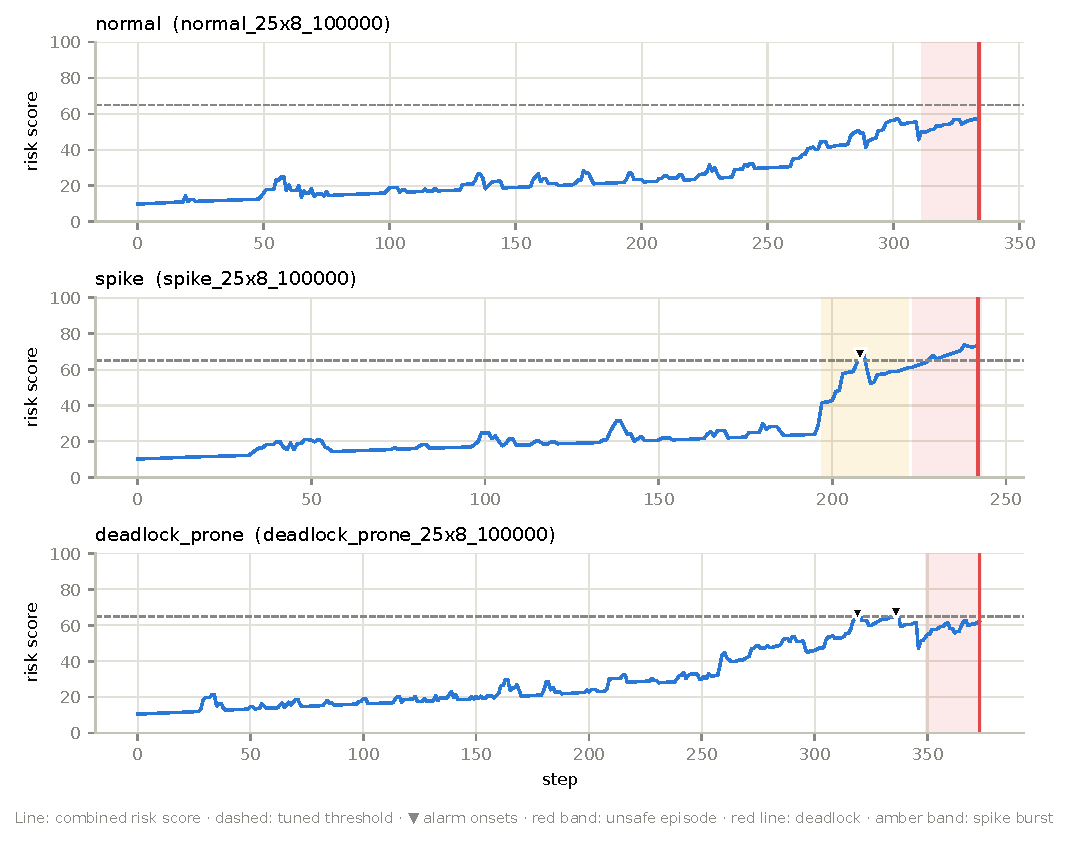
\includegraphics[width=0.92\textwidth]{fig1_timelines.pdf}
\caption{Example test sequences (25 processes, 8 resource types), one per workload. Blue: rule-based risk score; dashed: tuned threshold; triangles: alarm onsets; red band: unsafe episode; red line: deadlock; amber band: spike burst.}
\label{fig:timeline}
\end{figure*}

\begin{figure}[t]
\centering
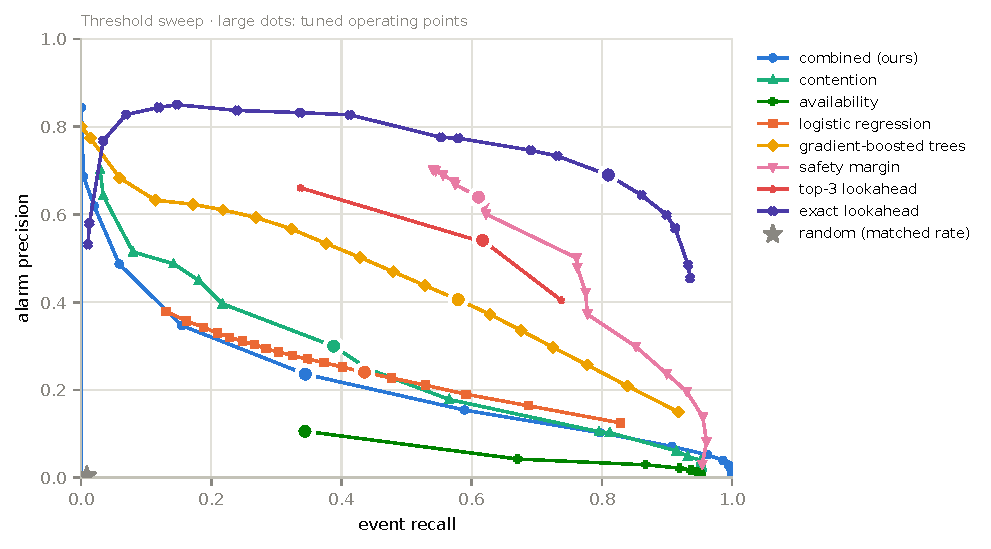
\includegraphics[width=\columnwidth]{fig3_pr_curves.pdf}
\caption{Precision--recall along each method's threshold sweep (plotted on test data, never used for selection; points are not interpolated~\cite{Davis2006}). Large dots: tuned operating points; star: random baseline.}
\label{fig:pr}
\end{figure}

\subsection{RQ4: which signals, which combination, and learned models}
Contention alone (F1 = \ContF) beat the weighted-mean score (\CombF); need pressure (\NeedF), waiting ratio (\WaitF) and request rate (\RateF) were weaker. The ablation (Table~\ref{tab:ablation}) shows that removing contention or request rate hurts the equal-weight mean most, while removing waiting ratio helps: averaging dilutes the strongest indicator, which is also why the tuner doubled contention's weight. The weighted maximum (\CMaxF) selected weights under which contention always decides, and so coincides with contention alone. Learned models on the same signals tell a sharper story. Logistic regression reached only \LrF, but gradient-boosted trees reached \GbtF{} with an NAB score of \GbtNab{} against \CombNab{} for the rule-based score, and on jointly captured onsets they warned earlier (median \PairGbtOther{} vs.\ \PairGbtComb{} steps). Since a linear model gains little and a tree ensemble gains much, the useful information lies in \emph{interactions} between the indicators---for example contention matters most when waiting is also rising---which a single weighted sum cannot express. The price is explainability: the rule-based score can name the indicator that triggered an alarm, the tree ensemble cannot.

\begin{table}[t]
\centering
\footnotesize
\caption{Ablation: combined score with one indicator removed (each re-tuned on the tuning split).}
\label{tab:ablation}
\begin{tabular}{lrrrr}
\toprule
variant & precision & recall & F1 & FA/1000 \\
\midrule
all five, equal & 0.17 & 0.40 & 0.24 & 0.59 \\
without scarcity & 0.19 & 0.39 & 0.26 & 0.47 \\
without need\_pressure & 0.17 & 0.45 & 0.25 & 0.64 \\
without contention & 0.14 & 0.36 & 0.20 & 0.65 \\
without waiting\_ratio & 0.23 & 0.31 & 0.27 & 0.30 \\
without request\_rate & 0.15 & 0.41 & 0.22 & 0.93 \\
\bottomrule
\end{tabular}
\end{table}


\subsection{RQ7a: the cost--accuracy frontier}
On the sequences where every method was computed (Table~\ref{tab:lookahead}), the state-based checks were the most accurate: exact lookahead reached F1 = \LookFsub, the safety margin \MargFsub{} and top-3 lookahead \ApprFsub, against \GbtFsub{} for boosted trees and \CombFsub{} for the rule-based score. Their costs differ by more than an order of magnitude (Table~\ref{tab:cost}, Fig.~\ref{fig:frontier}). The indicators and learned models need only a few vector operations per step. The safety margin costs \MargCostAll$\times$ a simulation step on average and \MargCostMaxN$\times$ at 200 processes, and top-3 lookahead \ApprCostAll$\times$ and \ApprCostMaxN$\times$, because both use a fixed number of safety checks. Exact lookahead needs one check per running process, \LookCostAll$\times$ on average and \LookCostMaxN$\times$ at 200 processes. The safety margin therefore recovers almost all of exact lookahead's accuracy at about a twenty-fifth of its cost on large systems. Accuracy is not the only axis: on jointly captured onsets the state-based checks warned later than the rule-based score (median \PairMargOther{} vs.\ \PairMargComb{} steps for the margin), and Fig.~\ref{fig:leadprec} shows that every method trades precision for lead time along its threshold sweep.

\begin{table}[t]
\centering
\footnotesize
\caption{All methods on the sequences where the lookahead baseline was computed.}
\label{tab:lookahead}
\begin{tabular}{lrrrr}
\toprule
method & precision & recall & F1 & lead med. \\
\midrule
combined (ours) & 0.56 & 0.37 & 0.44 [0.44, 0.45] & 5 \\
combined, max & 0.46 & 0.59 & 0.51 [0.51, 0.52] & 6 \\
need pressure & 0.65 & 0.11 & 0.18 [0.18, 0.19] & 4 \\
contention & 0.46 & 0.59 & 0.51 [0.51, 0.52] & 6 \\
waiting ratio & 0.32 & 0.09 & 0.14 [0.14, 0.15] & 4 \\
request rate & 0.44 & 0.27 & 0.33 [0.33, 0.34] & 8 \\
availability & 0.48 & 0.22 & 0.30 [0.29, 0.30] & 4 \\
logistic regr. & 0.23 & 0.79 & 0.36 [0.36, 0.37] & 12 \\
boosted trees & 0.40 & 0.81 & 0.54 [0.53, 0.54] & 10 \\
safety margin & 0.68 & 0.77 & 0.72 [0.71, 0.72] & 4 \\
top-3 lookahead & 0.63 & 0.77 & 0.69 [0.69, 0.70] & 5 \\
exact lookahead & 0.69 & 0.81 & 0.74 [0.74, 0.75] & 4 \\
random & 0.03 & 0.01 & 0.01 [0.01, 0.01] & 9 \\
\bottomrule
\end{tabular}
\end{table}


\begin{figure}[t]
\centering
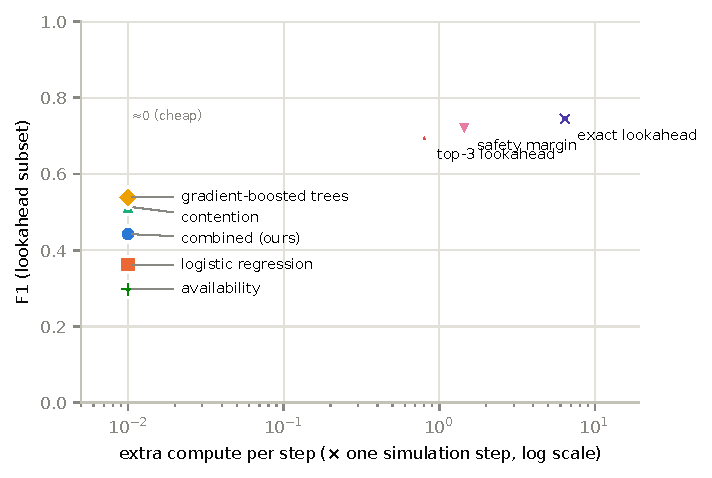
\includegraphics[width=\columnwidth]{fig9_cost_frontier.pdf}
\caption{Cost--accuracy frontier: F1 on the sequences where all methods were computed, against extra compute per step (relative to one simulation step, log scale). Cheap signals are drawn at the axis floor.}
\label{fig:frontier}
\end{figure}

\begin{table}[t]
\centering
\footnotesize
\caption{Measured compute per step (test split). A simulation step includes one safety check and the indicators; learned models add a few vector operations.}
\label{tab:cost}
\begin{tabular}{lrrr}
\toprule
computation & processes & $\mu$s/step & $\times$ simulation step \\
\midrule
simulation step & all & 289.18 & 1.00 \\
one safety check & all & 59.89 & 0.21 \\
safety margin & all & 417.28 & 1.44 \\
safety margin & 200 & 479.30 & 1.66 \\
top-3 lookahead & all & 231.46 & 0.80 \\
top-3 lookahead & 200 & 264.00 & 0.91 \\
exact lookahead & all & 1850.09 & 6.40 \\
exact lookahead & 200 & 12565.63 & 43.45 \\
\bottomrule
\end{tabular}
\end{table}


\begin{figure}[t]
\centering
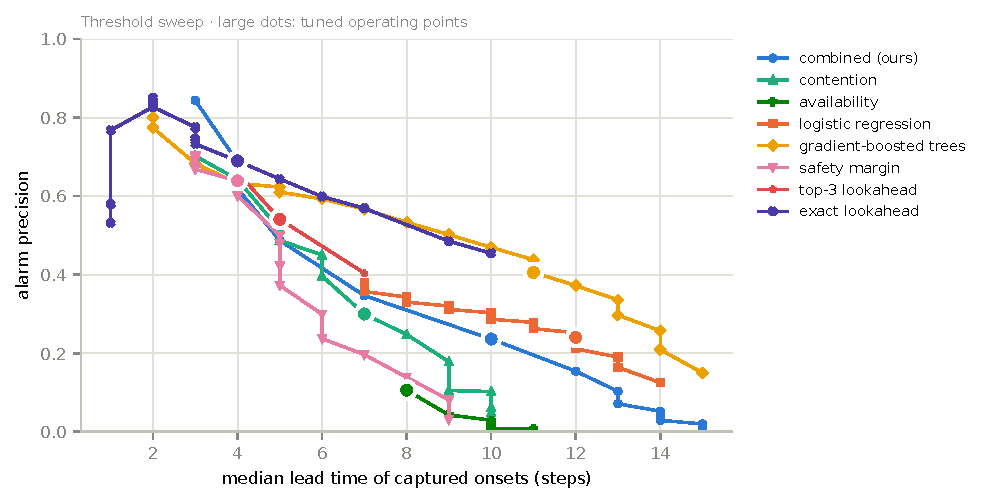
\includegraphics[width=\columnwidth]{fig10_precision_lead.pdf}
\caption{Alarm precision against median lead time along each method's threshold sweep~\cite{Munchmeyer2021}. Large dots: tuned operating points.}
\label{fig:leadprec}
\end{figure}

\subsection{RQ5: workloads}
Warning quality depends strongly on how danger builds (Fig.~\ref{fig:scen}, Table~\ref{tab:scenario}). Spike workloads were easiest for the rule-based score (F1 = \CombFSpike): bursts raise several indicators at once, and unsafe onsets followed a median \SpikeMedSteps{} steps after the burst began (only \SpikeBefore\% occurred before it). Gradual build-ups were harder (\CombFNormal{} for normal and \CombFDlp{} for deadlock-prone workloads); there, waiting ratio alone (\WaitFNormal, \WaitFDlp) beat the weighted mean, and the state-based checks degraded least (safety margin \MargFNormal{} and \MargFDlp), because they test the safety boundary directly instead of inferring it from aggregates.

\begin{figure}[t]
\centering
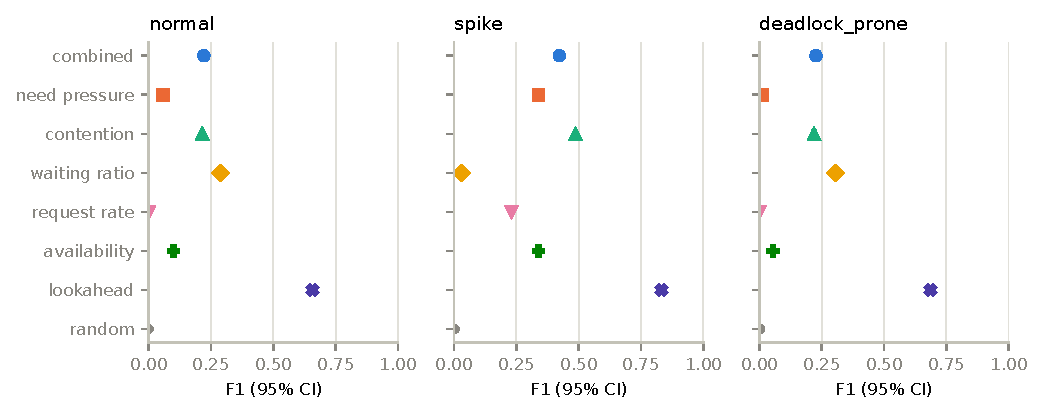
\includegraphics[width=\columnwidth]{fig4_per_scenario_f1.pdf}
\caption{F1 per workload with 95\% bootstrap confidence intervals.}
\label{fig:scen}
\end{figure}
\begin{table}[t]
\centering
\footnotesize
\caption{F1 per scenario (unsafe target, $H_{max}=20$).}
\label{tab:scenario}
\begin{tabular}{lrrr}
\toprule
method & deadlock\_prone & spike & normal \\
\midrule
combined & 0.23 & 0.42 & 0.22 \\
need\_pressure & 0.01 & 0.34 & 0.06 \\
contention & 0.22 & 0.49 & 0.21 \\
waiting\_ratio & 0.31 & 0.03 & 0.29 \\
request\_rate & 0.00 & 0.23 & 0.00 \\
availability & 0.05 & 0.34 & 0.10 \\
lookahead & 0.69 & 0.83 & 0.66 \\
random & 0.01 & 0.01 & 0.00 \\
\bottomrule
\end{tabular}
\end{table}


\subsection{RQ6: unsafe versus deadlock}
In our model unsafe episodes rarely recover: \EpDeadSpike\% of resolved episodes ended in deadlock under spike and \EpDeadDlp\% under deadlock-prone workloads, and \EpDeadNormal\% under normal workloads, where early releases allow some recovery (Fig.~\ref{fig:episodes}). Processes eventually request their full claims, so Banker's worst-case assumption is realised. For the deadlock target, alarms are not suppressed during unsafe periods (Table~\ref{tab:deadlock}). With a 20-step horizon, waiting ratio and boosted trees anticipated deadlock best (F1 = \WaitFdl{} and \GbtFdl), since blocked processes accumulate as a deadlock forms; with a 50-step horizon exact lookahead led (\LookFdlL{} on its subset).

\begin{figure}[t]
\centering
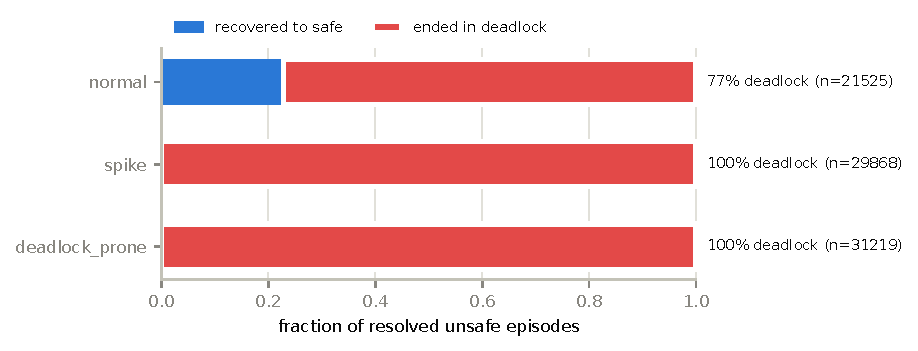
\includegraphics[width=0.9\columnwidth]{fig6_episode_outcomes.pdf}
\caption{Outcome of resolved unsafe episodes per workload.}
\label{fig:episodes}
\end{figure}
\begin{table}[t]
\centering
\footnotesize
\caption{Deadlock-onset target ($H_{max}=20$, alarms not masked while unsafe).}
\label{tab:deadlock}
\begin{tabular}{lrrrrr}
\toprule
method & precision & recall & F1 & lead med. & events \\
\midrule
combined (ours) & 0.21 & 0.71 & 0.33 & 13 & 77{,}700 \\
combined, max & 0.17 & 0.54 & 0.26 & 12 & 77{,}700 \\
need pressure & 0.18 & 0.34 & 0.23 & 10 & 77{,}700 \\
contention & 0.17 & 0.54 & 0.26 & 12 & 77{,}700 \\
waiting ratio & 0.33 & 0.83 & 0.48 & 12 & 77{,}700 \\
request rate & 0.07 & 0.06 & 0.06 & 15 & 77{,}700 \\
availability & 0.10 & 0.52 & 0.16 & 10 & 77{,}700 \\
logistic regr. & 0.18 & 0.65 & 0.29 & 14 & 77{,}700 \\
boosted trees & 0.31 & 0.99 & 0.48 & 14 & 77{,}700 \\
safety margin & 0.14 & 0.17 & 0.16 & 14 & 77{,}700 \\
top-3 lookahead & 0.11 & 0.15 & 0.13 & 15 & 77{,}700 \\
exact lookahead & 0.32 & 0.43 & 0.37 & 15 & 25{,}862 \\
random & 0.00 & 0.01 & 0.01 & 10 & 77{,}700 \\
\bottomrule
\end{tabular}
\end{table}


\subsection{RQ8: misdeclared claims}
Banker's algorithm needs declared maximum claims, which real systems rarely know. We fed the tuned rules indicators computed from claims misdeclared by up to $\pm$20\% per entry while the ground truth used the true claims (Table~\ref{tab:robust}, Fig.~\ref{fig:robust}). F1 changed by at most half a percentage point for every method (\CombFdelta{} for the rule-based score, \ContFdelta{} for contention, \GbtFdelta{} for boosted trees). The indicators aggregate need over all processes and resource types, so per-entry claim errors largely cancel; this partly answers the objection that Banker-style signals require exactly known claims.

\begin{table}[t]
\centering
\footnotesize
\caption{Robustness: the same tuned rules when need pressure and contention are computed from maximum claims misdeclared by up to $\pm$20\% (ground truth uses the true claims).}
\label{tab:robust}
\begin{tabular}{lrrr}
\toprule
method & F1, true claims & F1, claims $\pm$20\% & change \\
\midrule
combined (ours) & 0.280 & 0.280 & +0.000 \\
combined, max & 0.338 & 0.337 & -0.001 \\
need pressure & 0.190 & 0.194 & +0.004 \\
contention & 0.338 & 0.337 & -0.001 \\
logistic regr. & 0.310 & 0.311 & +0.002 \\
boosted trees & 0.477 & 0.476 & -0.001 \\
\bottomrule
\end{tabular}
\end{table}

\begin{figure}[t]
\centering
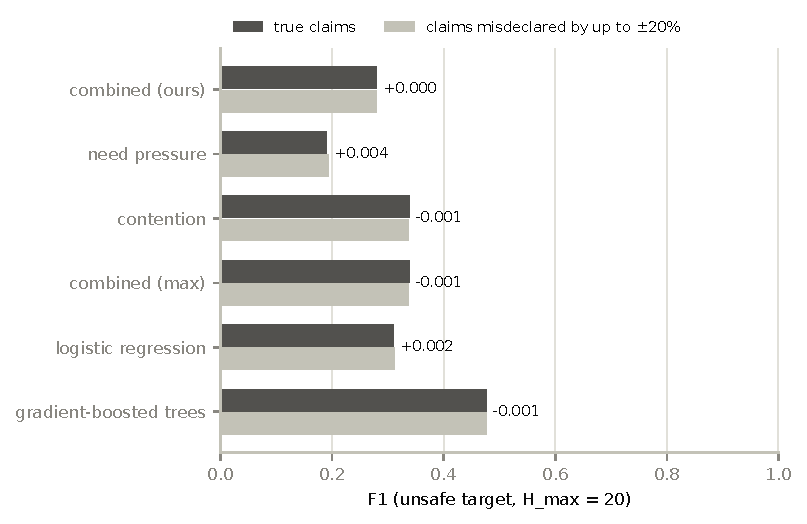
\includegraphics[width=0.9\columnwidth]{fig11_robustness.pdf}
\caption{F1 with true and with misdeclared ($\pm$20\%) maximum claims, using the same tuned rules.}
\label{fig:robust}
\end{figure}

\subsection{Sensitivity to the warning horizon}
With the same alarms, widening the horizon raises F1 for every method (rule-based score: \CombFHFive, \CombFHTen, \CombFHTwenty{} and \CombFHFifty{} for $H_{\max}$ = 5, 10, 20, 50; Fig.~\ref{fig:hmax}), showing that many alarms precede onsets by more than 20 steps.

\begin{figure}[t]
\centering
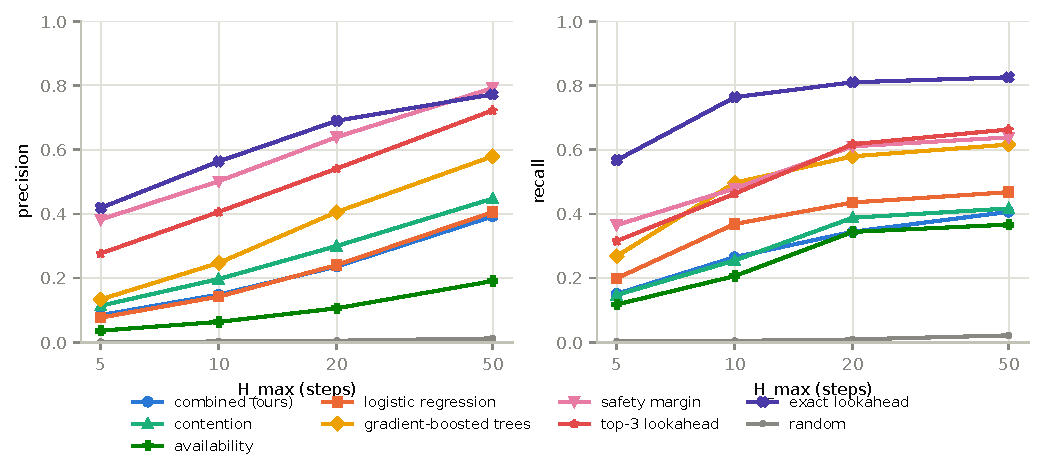
\includegraphics[width=\columnwidth]{fig5_hmax_sensitivity.pdf}
\caption{Precision and recall as the warning horizon $H_{\max}$ varies (same alarms).}
\label{fig:hmax}
\end{figure}

\subsection{RQ7b: scaling of the safety check}
The vectorised safety check was \SpeedupMin$\times$ (10 processes) to \SpeedupMax$\times$ (\ScaleMaxN{} processes) faster than the textbook loop (Table~\ref{tab:scaling}, Fig.~\ref{fig:scaling}). Measured growth with $n$ was far below the $\Theta(mn^2)$ worst case (log--log slopes \SlopeVec{} vectorised and \SlopeRef{} reference at $m=20$): realistic states clear in a few passes, consistent with Belik's observation that typical cases are cheaper than the worst case~\cite{Belik1987}.

\begin{table}[!htb]
\centering
\footnotesize
\caption{Runtime scaling: time per Banker's safety check on random valid states (vectorised vs. reference) and whole-simulator time per step.}
\label{tab:scaling}
\begin{tabular}{lrrrrr}
\toprule
n & m & vec $\mu$s & ref $\mu$s & speed-up & $\mu$s/step \\
\midrule
10 & 5 & 7.1 & 9.7 & 1.4 & 100.7 \\
10 & 10 & 6.9 & 9.4 & 1.4 & 103.0 \\
10 & 20 & 6.9 & 10.5 & 1.5 & 103.7 \\
25 & 5 & 9.0 & 19.5 & 2.2 & 101.2 \\
25 & 10 & 7.4 & 17.6 & 2.4 & 104.6 \\
25 & 20 & 7.4 & 17.3 & 2.3 & 107.5 \\
50 & 5 & 9.1 & 29.6 & 3.3 & 102.1 \\
50 & 10 & 8.1 & 28.4 & 3.5 & 113.3 \\
50 & 20 & 9.0 & 28.6 & 3.2 & 118.8 \\
100 & 5 & 12.1 & 60.8 & 5.0 & 110.0 \\
100 & 10 & 9.9 & 51.9 & 5.3 & 118.0 \\
100 & 20 & 11.2 & 54.3 & 4.9 & 118.9 \\
200 & 5 & 17.8 & 138.0 & 7.7 & 129.1 \\
200 & 10 & 13.7 & 103.3 & 7.6 & 131.7 \\
200 & 20 & 15.6 & 99.7 & 6.4 & 141.6 \\
\bottomrule
\end{tabular}
\end{table}

\begin{figure}[t]
\centering
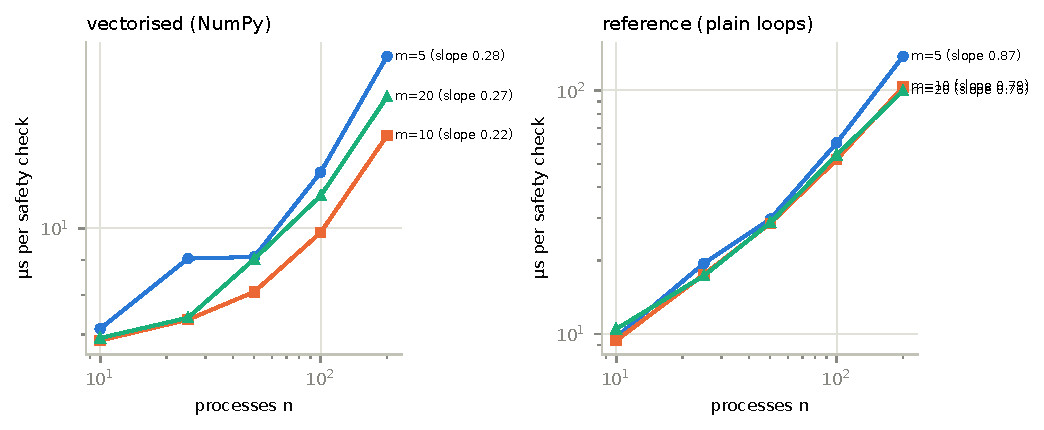
\includegraphics[width=\columnwidth]{fig7_scaling.pdf}
\caption{Time per safety check versus number of processes (log--log), vectorised and reference implementations.}
\label{fig:scaling}
\end{figure}

% ===================================================================
\section{Discussion}
\textbf{Circularity.} The indicators, the learned models and Banker's check all read the same allocation state, so some correlation is built in. That is the point of the question: can cheap aggregates of that state anticipate an expensive verdict before it flips? The baselines bound the answer from both sides---random alarms and the free-resource rule from below, exact lookahead from above---and the state-based checks show how much of the information in the state cheap aggregates leave unused.

\textbf{A frontier, not a winner.} No method dominates on accuracy, cost, lead time and explainability at once. The rule-based score is cheap and fully explainable but only moderately precise; boosted trees on the same cheap signals are markedly better and warn early but are opaque; the safety margin is nearly as accurate as exact lookahead at a fraction of its cost but warns later. A practical design follows directly: run a cheap score continuously and invoke the safety margin, or exact lookahead on small systems, only when the score is elevated, paying the safety-check cost only in risky periods.

\textbf{Explainability.} A rule-based alarm can be traced to the indicator that triggered it, which matters for alerts that page humans~\cite{Ewaschuk2016SRE}.

% ===================================================================
\section{Threats to Validity}
\textbf{Synthetic workloads.} Workloads are synthetic; we mitigate this with three controlled patterns, one modelled on reported gang-scheduling behaviour~\cite{Jayaram2019FfDL}, and per-workload reporting. \textbf{Known claims.} Banker's algorithm needs declared maximum claims~\cite{Dijkstra-EWD623}, an inherited limitation also noted for DBDAA~\cite{Zohora2024}; we quantify sensitivity to misdeclared claims. \textbf{Calibration.} Claim tightness, which largely decides whether a workload becomes unsafe, was calibrated for class balance on tuning seeds. \textbf{Modelling choices.} Flicker merging, the warm-up exclusion, the refractory period and ending a sequence at the first (possibly partial) deadlock are design decisions taken from early-warning practice~\cite{Hyland2020,Tatbul2018}; the horizon study shows their direction of effect. \textbf{Subset comparison.} Exact lookahead was computed on a seed subset for large systems; we therefore compare all methods on that same subset. \textbf{Dependence.} Steps within a sequence are correlated, so the bootstrap resamples whole sequences.

% ===================================================================
\section{Conclusion and Future Work}
Simple, explainable indicators anticipate Banker-unsafe states several steps ahead, clearly better than chance and than a free-resource rule, at negligible cost and robustly to misdeclared claims. A non-linear model on the same signals improves accuracy substantially, showing that indicator interactions matter, and a scalar safety margin nearly matches exact lookahead at a small, size-independent number of safety checks. Together these results map the cost--accuracy--lead-time frontier for anticipating Banker's verdict. Future work includes two-stage warning (cheap score gating a lookahead), evaluation on real allocation traces, estimating claims rather than assuming them, incremental safety checks~\cite{Belik1987,Finkel1987,Zohora2024}, and an avoidance variant that acts on warnings.

\bibliographystyle{IEEEtran}
\bibliography{refs}

\end{document}
